\section{Resultados}
%Deben incluir los resultados de los experimentos, utilizando el formato más adecuado
%para su presentación. Deberón especificar claramente a qué experiencia corresponde
%cada resultado. No se incluirán aquí corridas de máquina. Algo fundamental en su
%aprendizaje en la materia es la presentación de resultados de forma clara y concisa para
%el lector.

% TASA DE EFICIENCIA EN FUNCIÓN DE LA CANTIDAD DE COMPONENTES PRINCIPALES TOMADAS
\subsection{Test de tasa de eficiencia en función de la cantidad de componentes principales consideradas}
\begin{figure}[H]{}
\centering
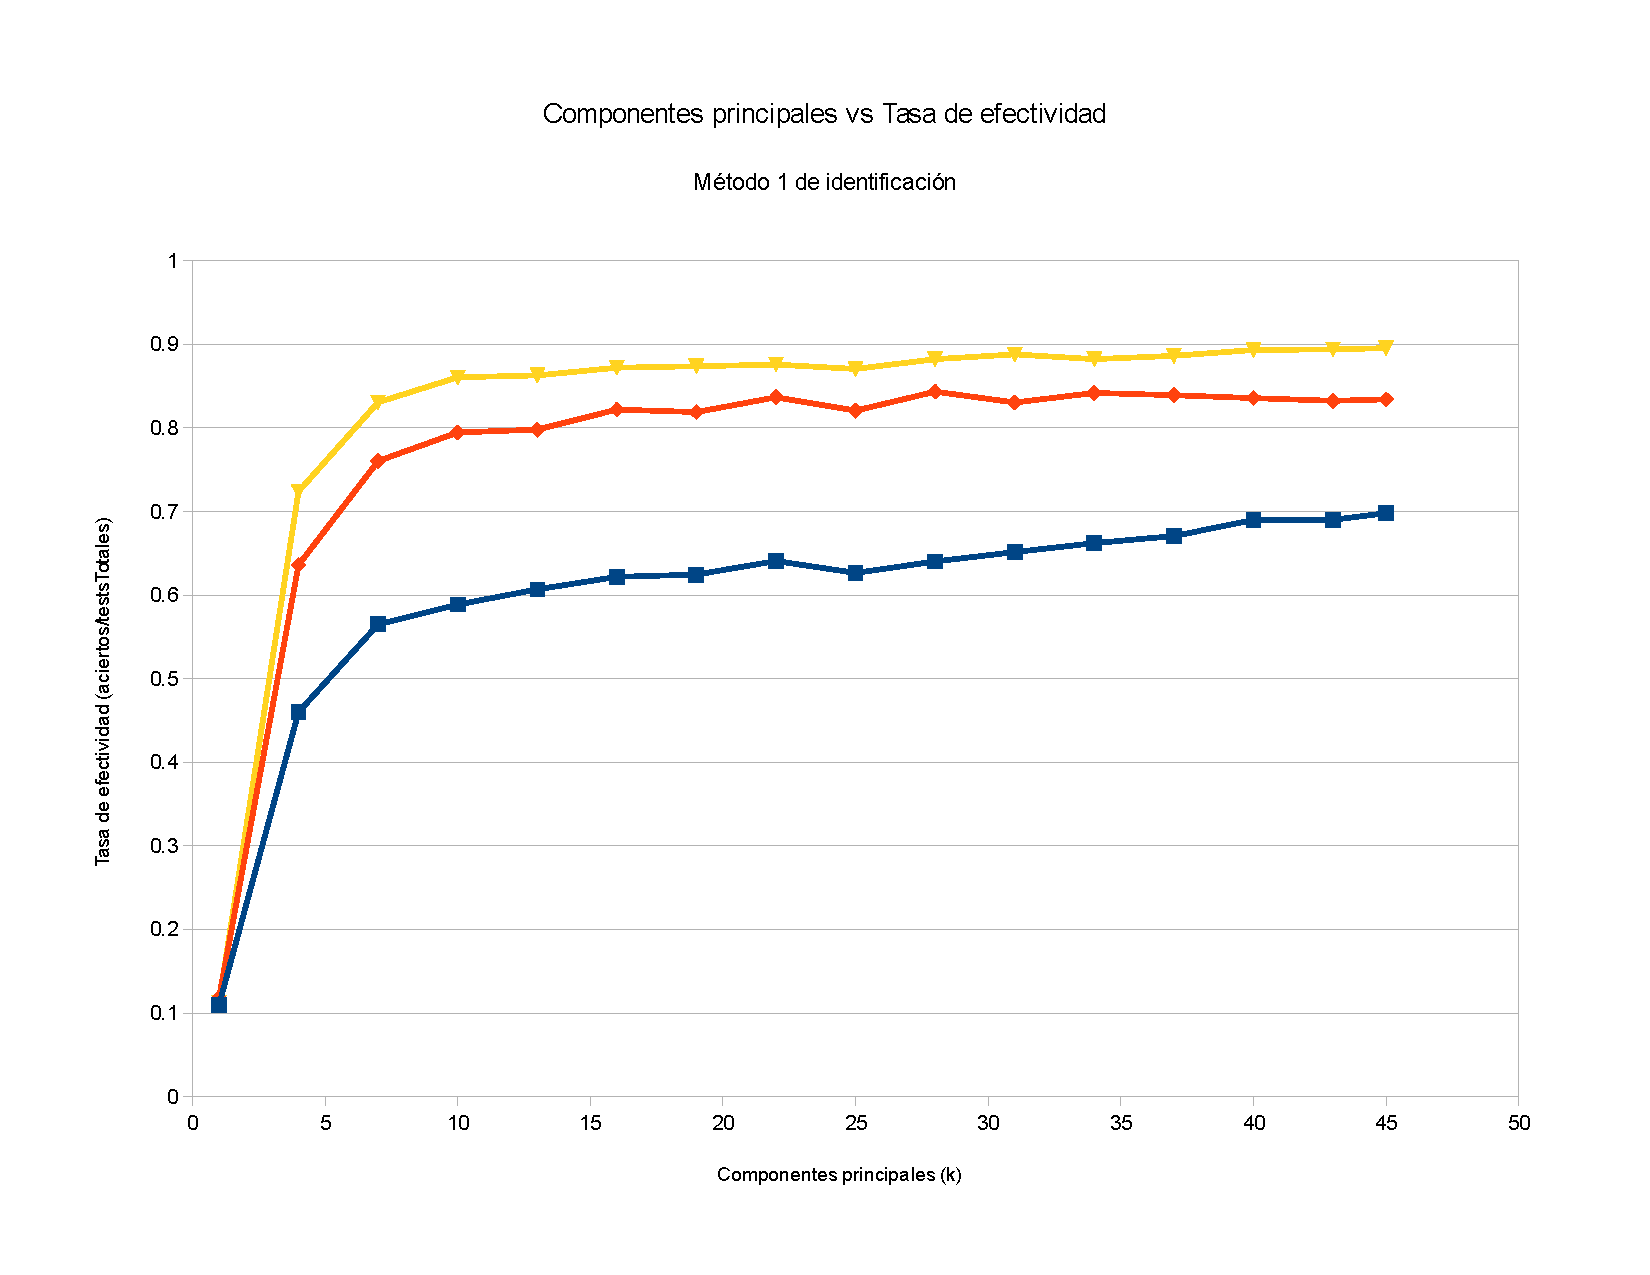
\includegraphics[scale=0.5]{graphs/componentesPrincipalesVsTasaDeEfectividadM1.pdf}
\caption{El método 1 de identificación se corresponde con el de Distancia Mínima}
\label{CPvsTE}
\end{figure}

Línea azul: $nimgp = 3$. Línea roja: $nimgp = 6$. Línea amarilla: $nimgp = 9$.

% TASA DE EFICIENCIA EN FUNCIÓN DE LA CANTIDAD DE SUJETOS CONSIDERADOS
\subsection{Test de tasa de eficiencia en función de la cantidad de personas}
\begin{figure}[H]{}
\centering
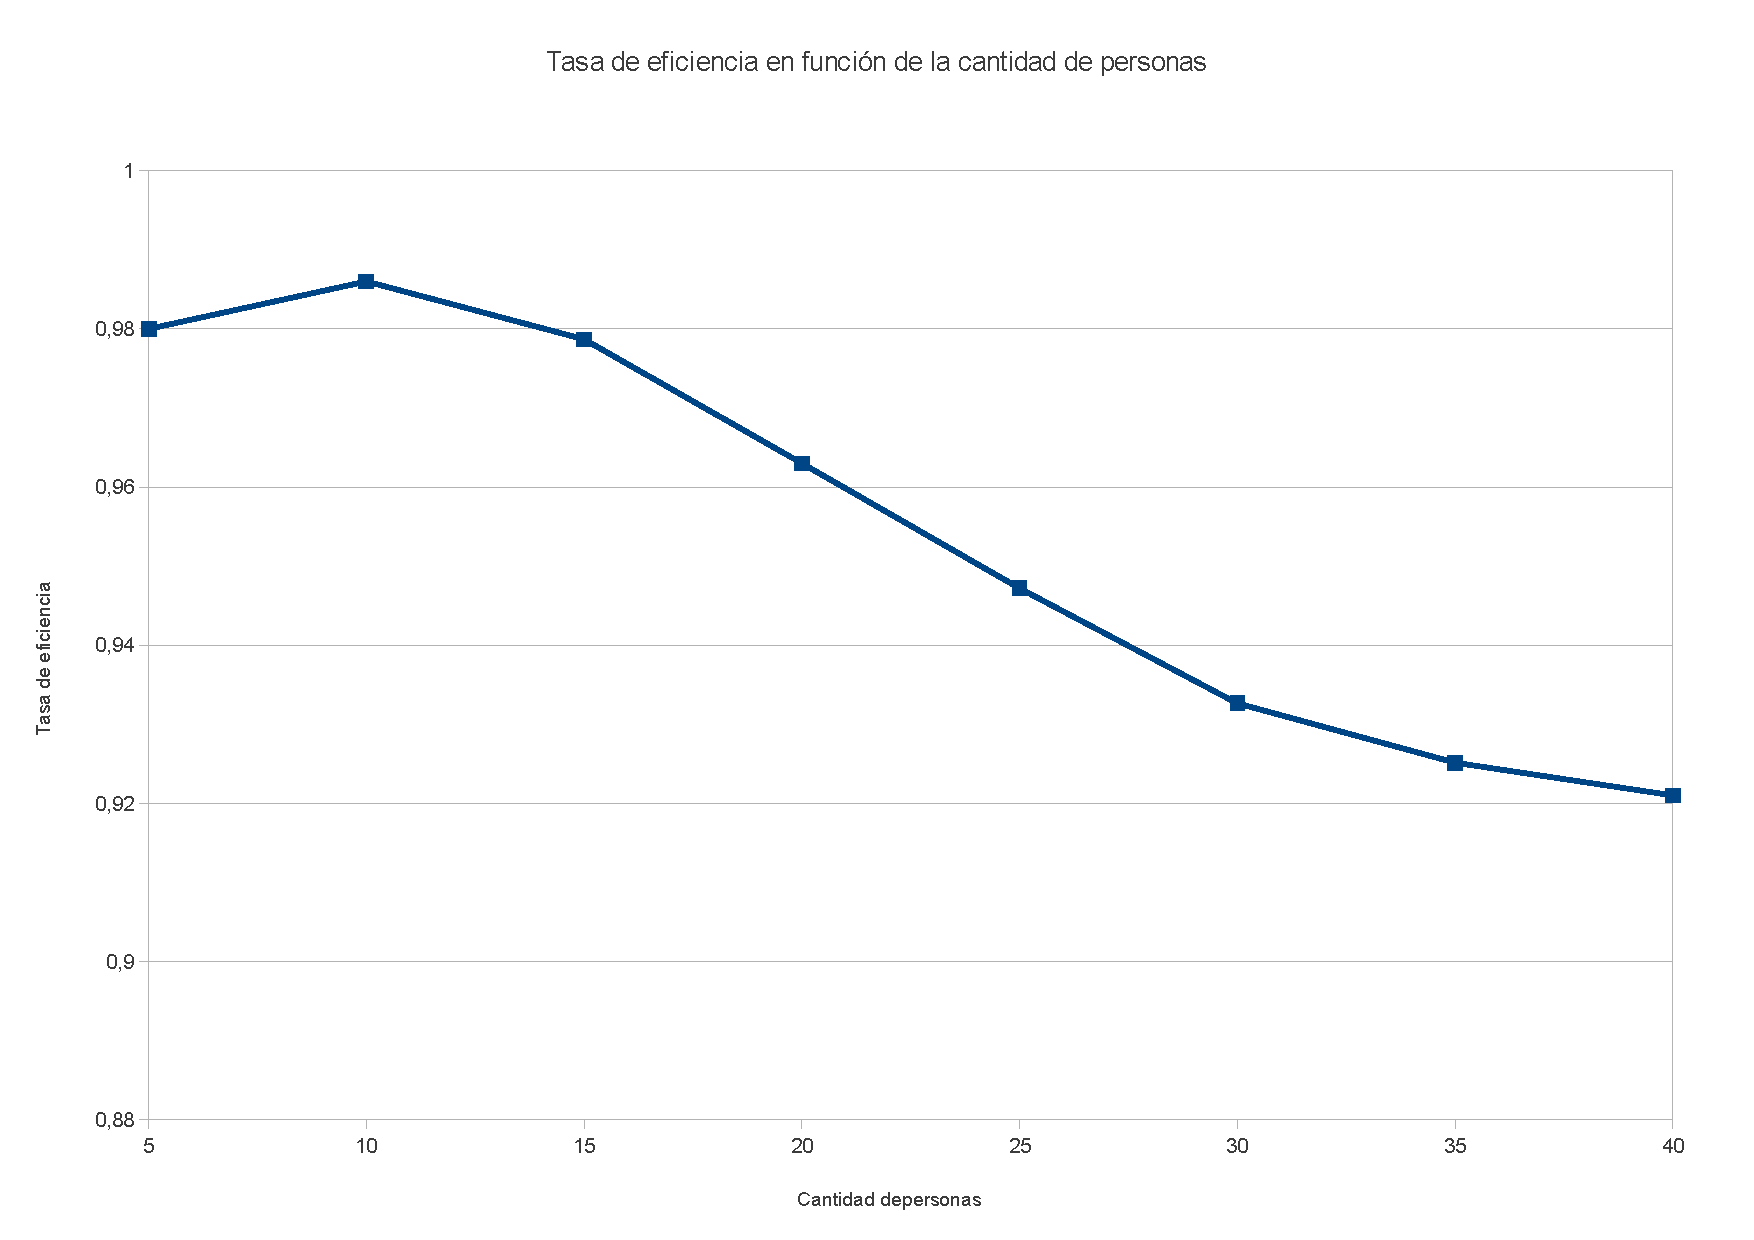
\includegraphics[scale=0.5]{graphs/CPvsTE.pdf}
\caption{Tasa de eficiencia en función de la cantidad de personas.}
\label{CPvsTE}
\end{figure}

% TASA DE EFICIENCIA EN FUNCIÓN DE nimgp
\subsection{Test de tasa de eficiencia en función de nimgp}
\begin{figure}[H]{}
\centering
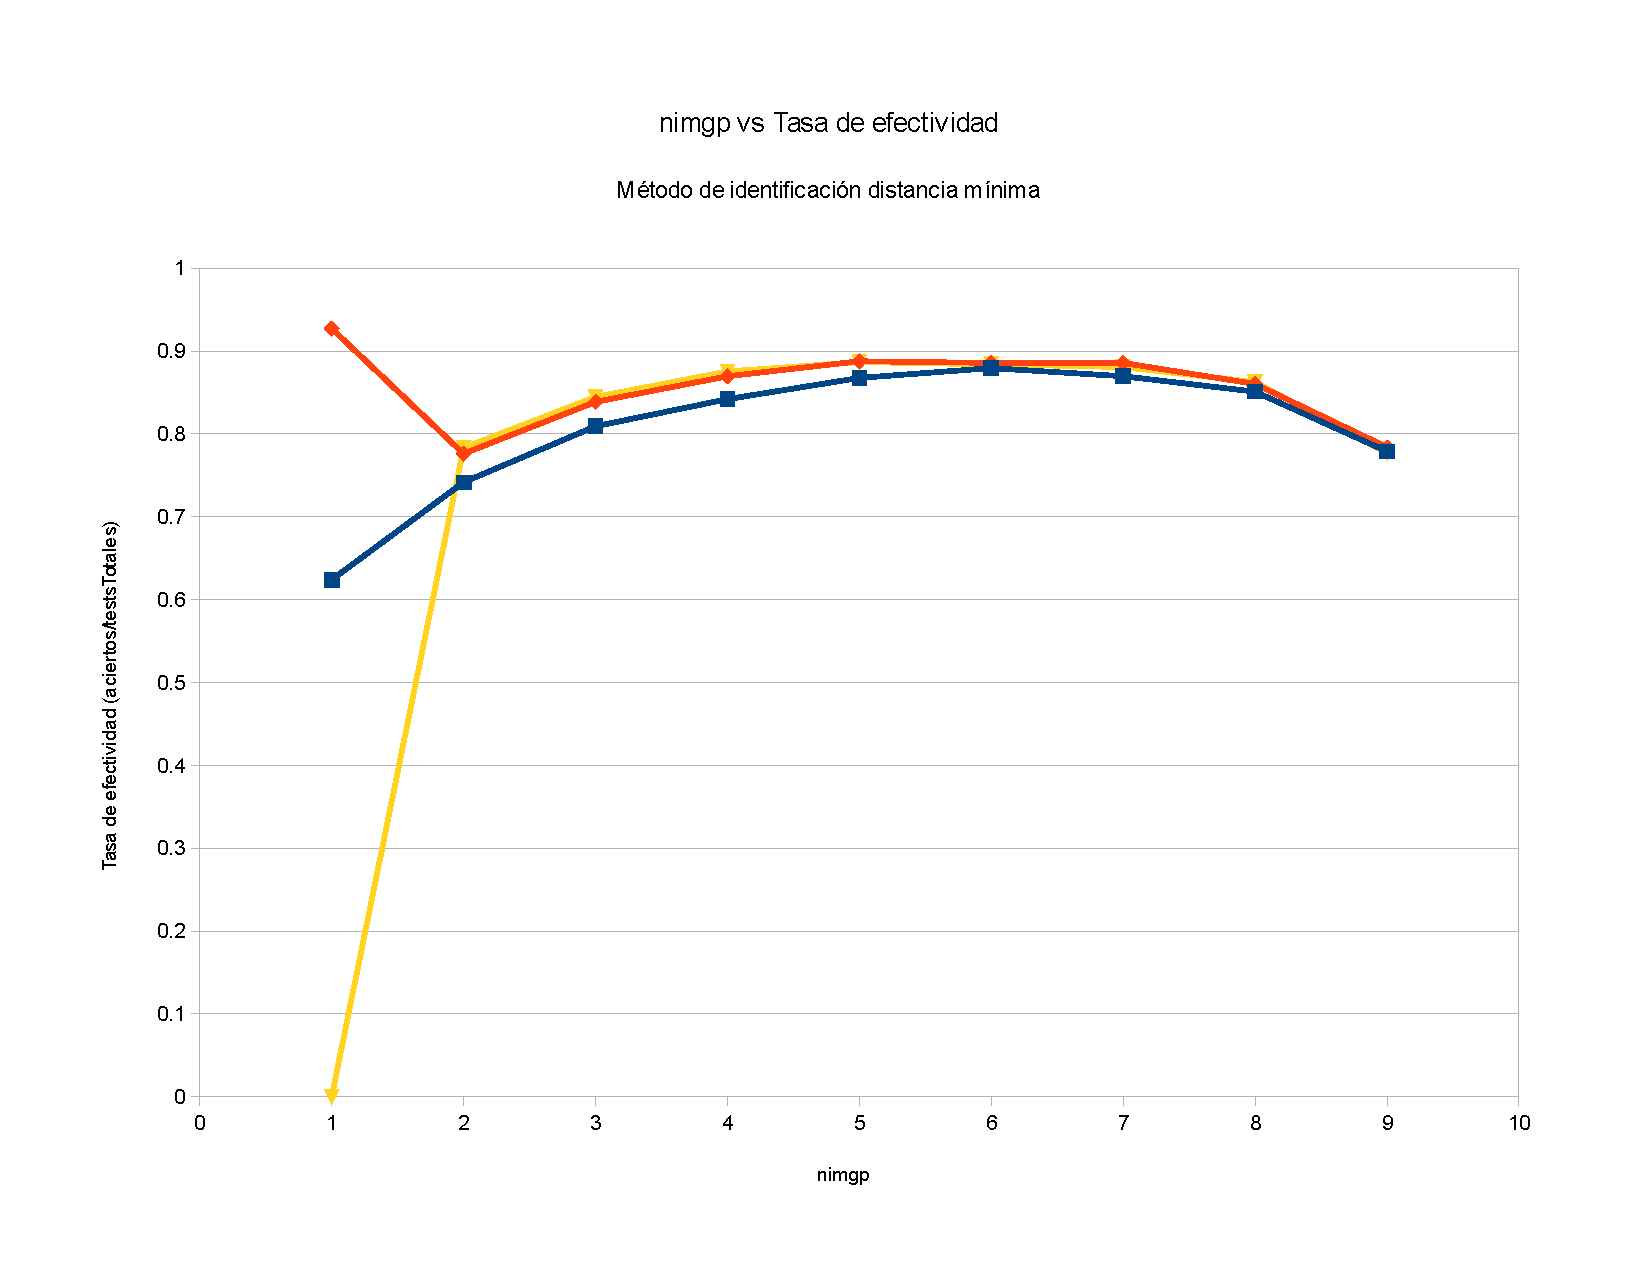
\includegraphics[scale=0.5]{graphs/nimgpVsTasaDeEfectividad.pdf}
\caption{Se graficó para 15, 30 y 45 componentes principales}
\label{nimgpvsTE}
\end{figure}

Línea azul: $k = 15$. Línea roja: $k = 30$. Línea amarilla: $k = 45$.

% TASA DE EFICIENCIA EN FUNCIÓN DE LA CANTIDAD DE COMPONENTES PRINCIPALES TOMADAS
\subsection{Test de comparación de los métodos de identificación}
\begin{figure}[H]{}
\centering
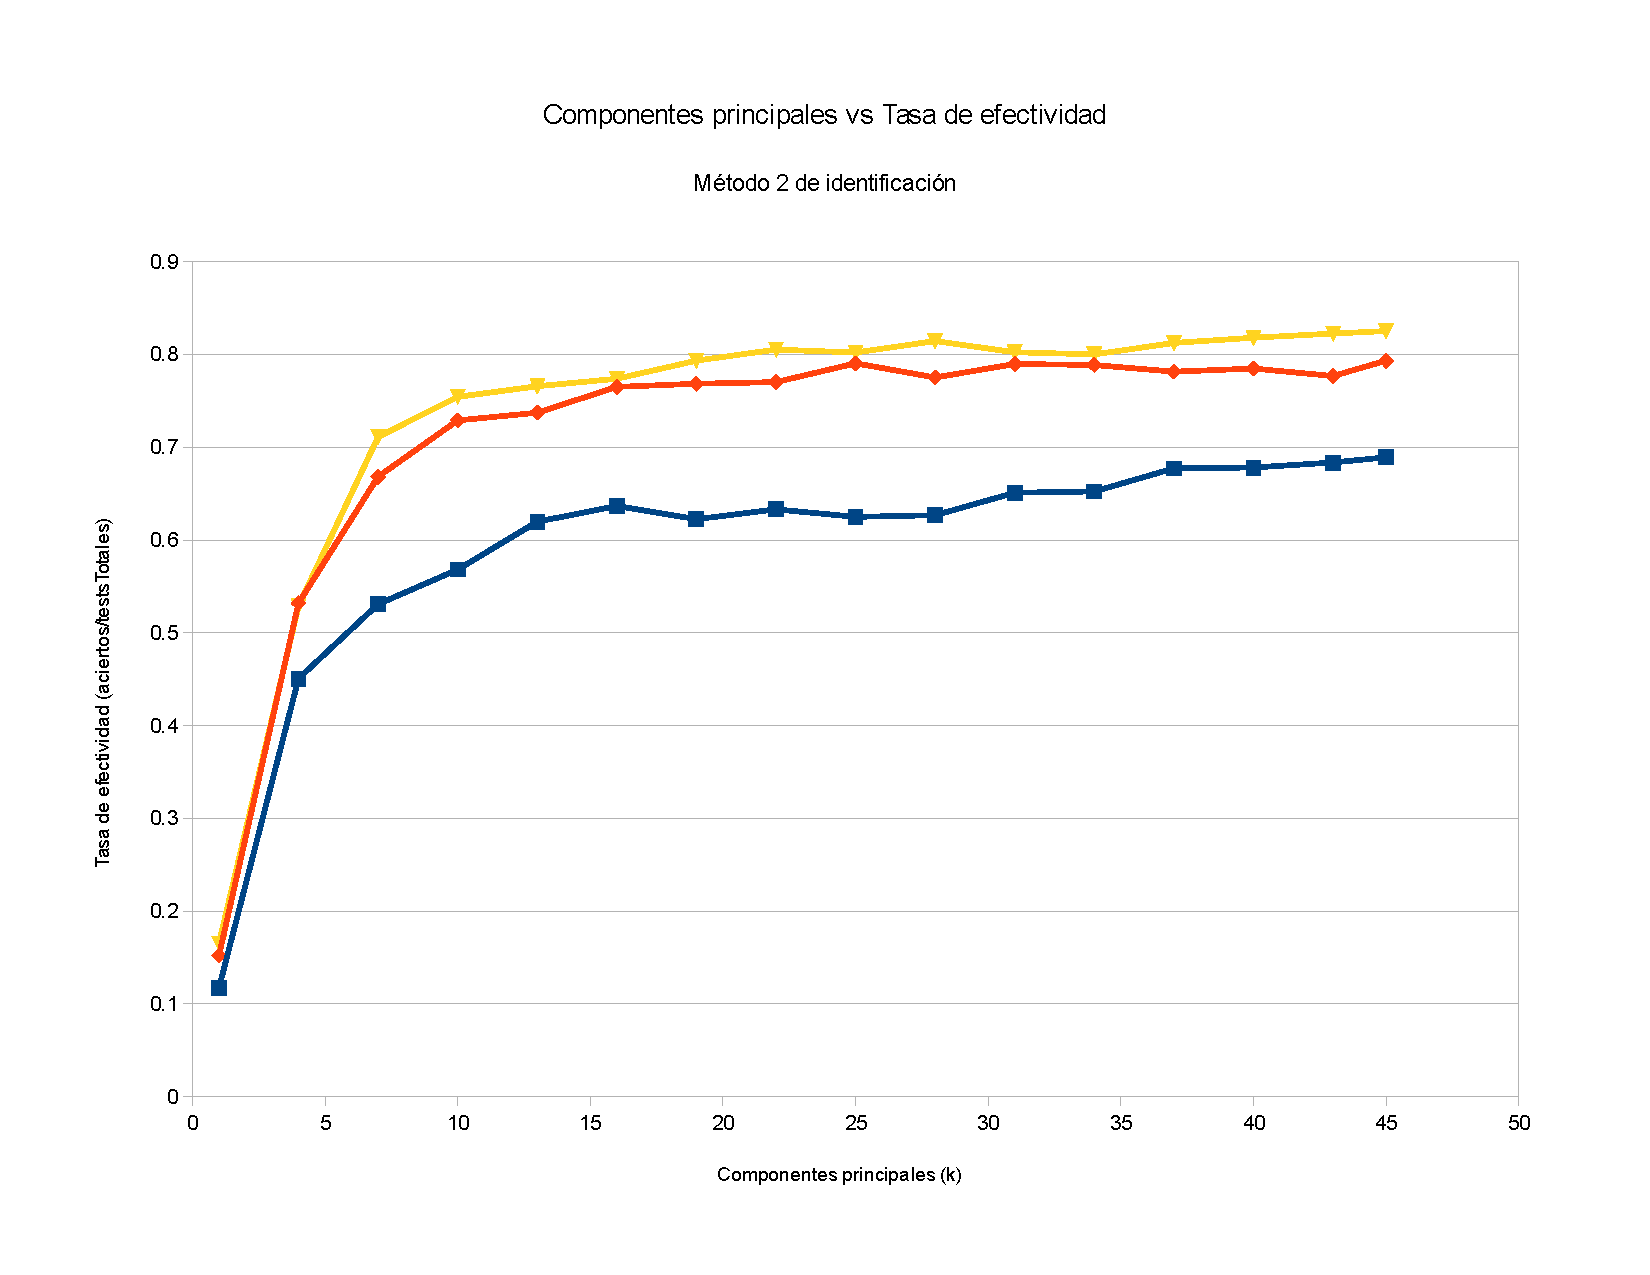
\includegraphics[scale=0.5]{graphs/componentesPrincipalesVsTasaDeEfectividadM2.pdf}
\caption{El método 2 de identificación se corresponde con el de Distancia Mínima Promedio}
\label{CPvsTE}
\end{figure}

Línea azul: $nimgp = 3$. Línea roja: $nimgp = 6$. Línea amarilla: $nimgp = 9$.

\subsection{Test de comparación de los métodos de identificación}
\begin{figure}[H]{}
\centering
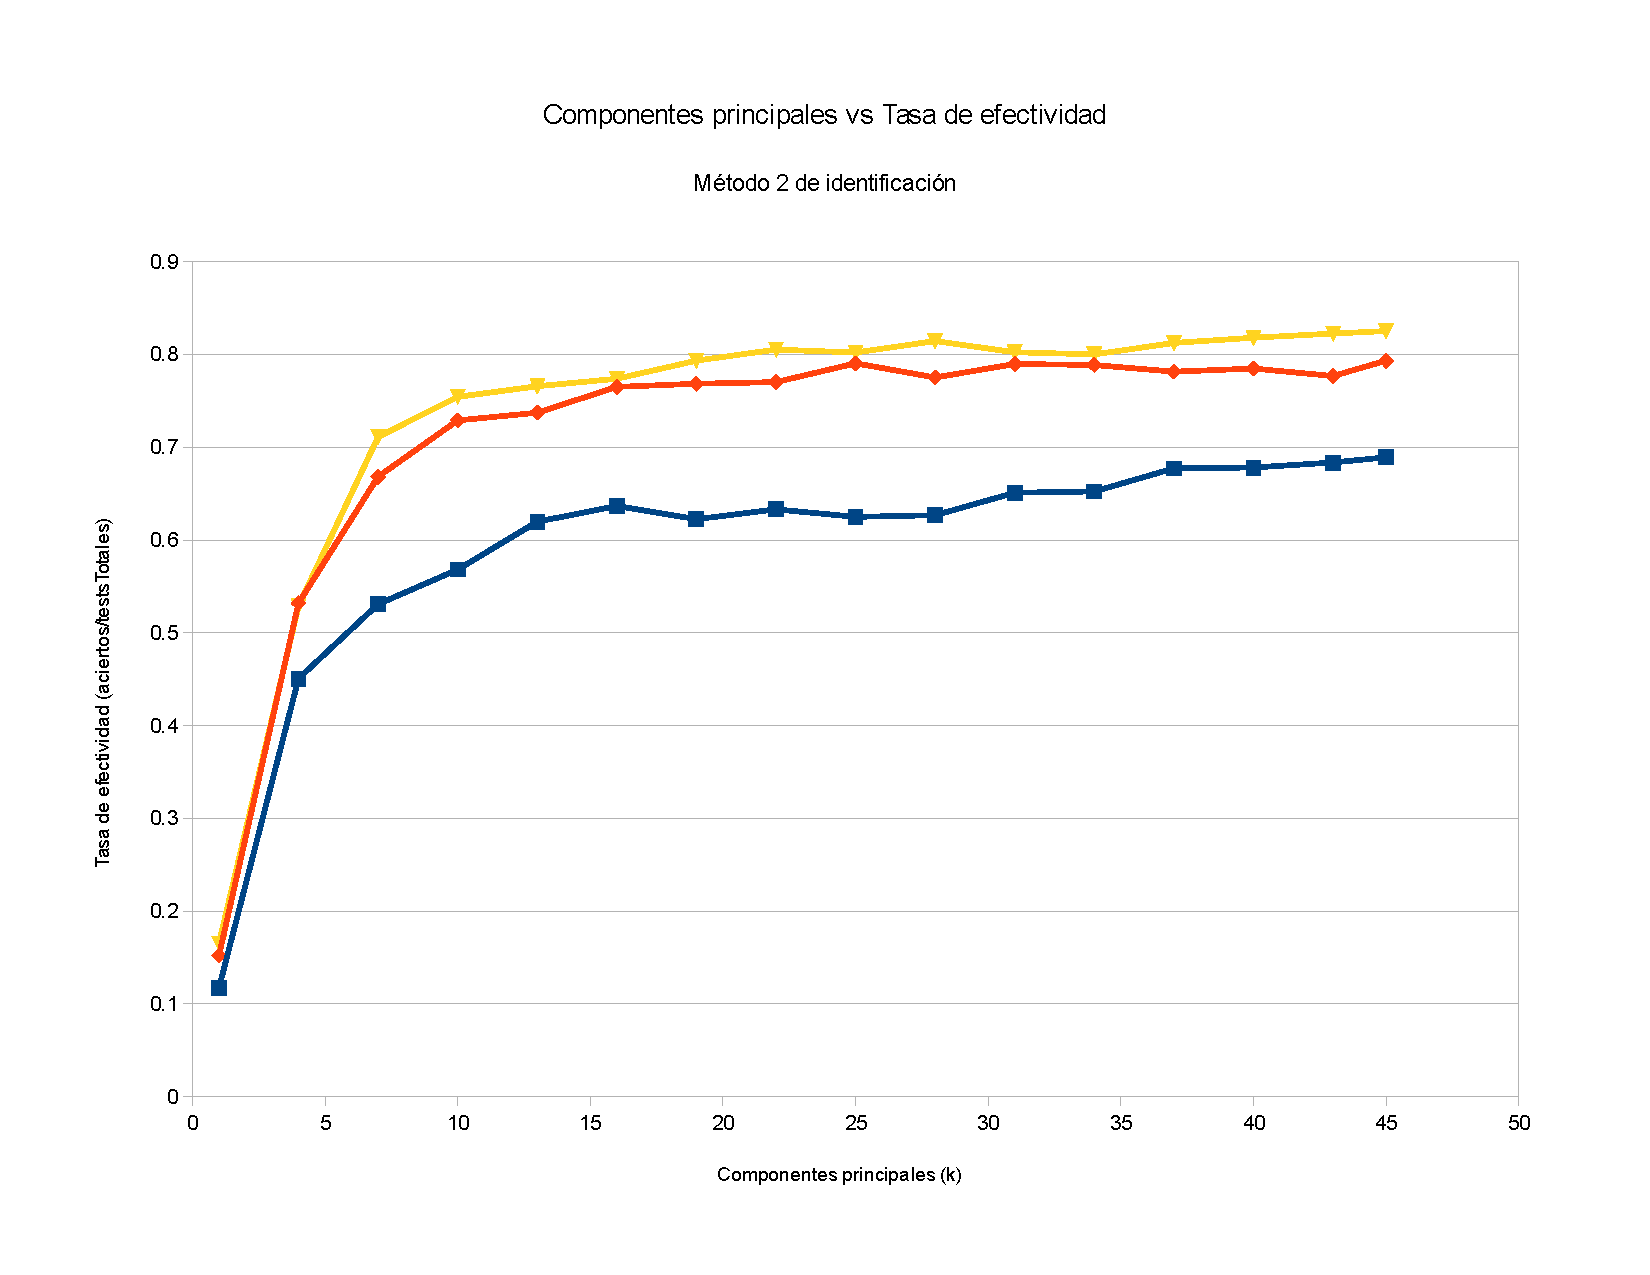
\includegraphics[scale=0.5]{graphs/componentesPrincipalesVsTasaDeEfectividadM2.pdf}
\caption{El método 2 de identificación se corresponde con el de Distancia Mínima Promedio}
\label{CPvsTE}
\end{figure}

\subsection{Test de tasa de eficiencia en función de la resolución de las imágenes}
\begin{figure}[H]{}
\centering
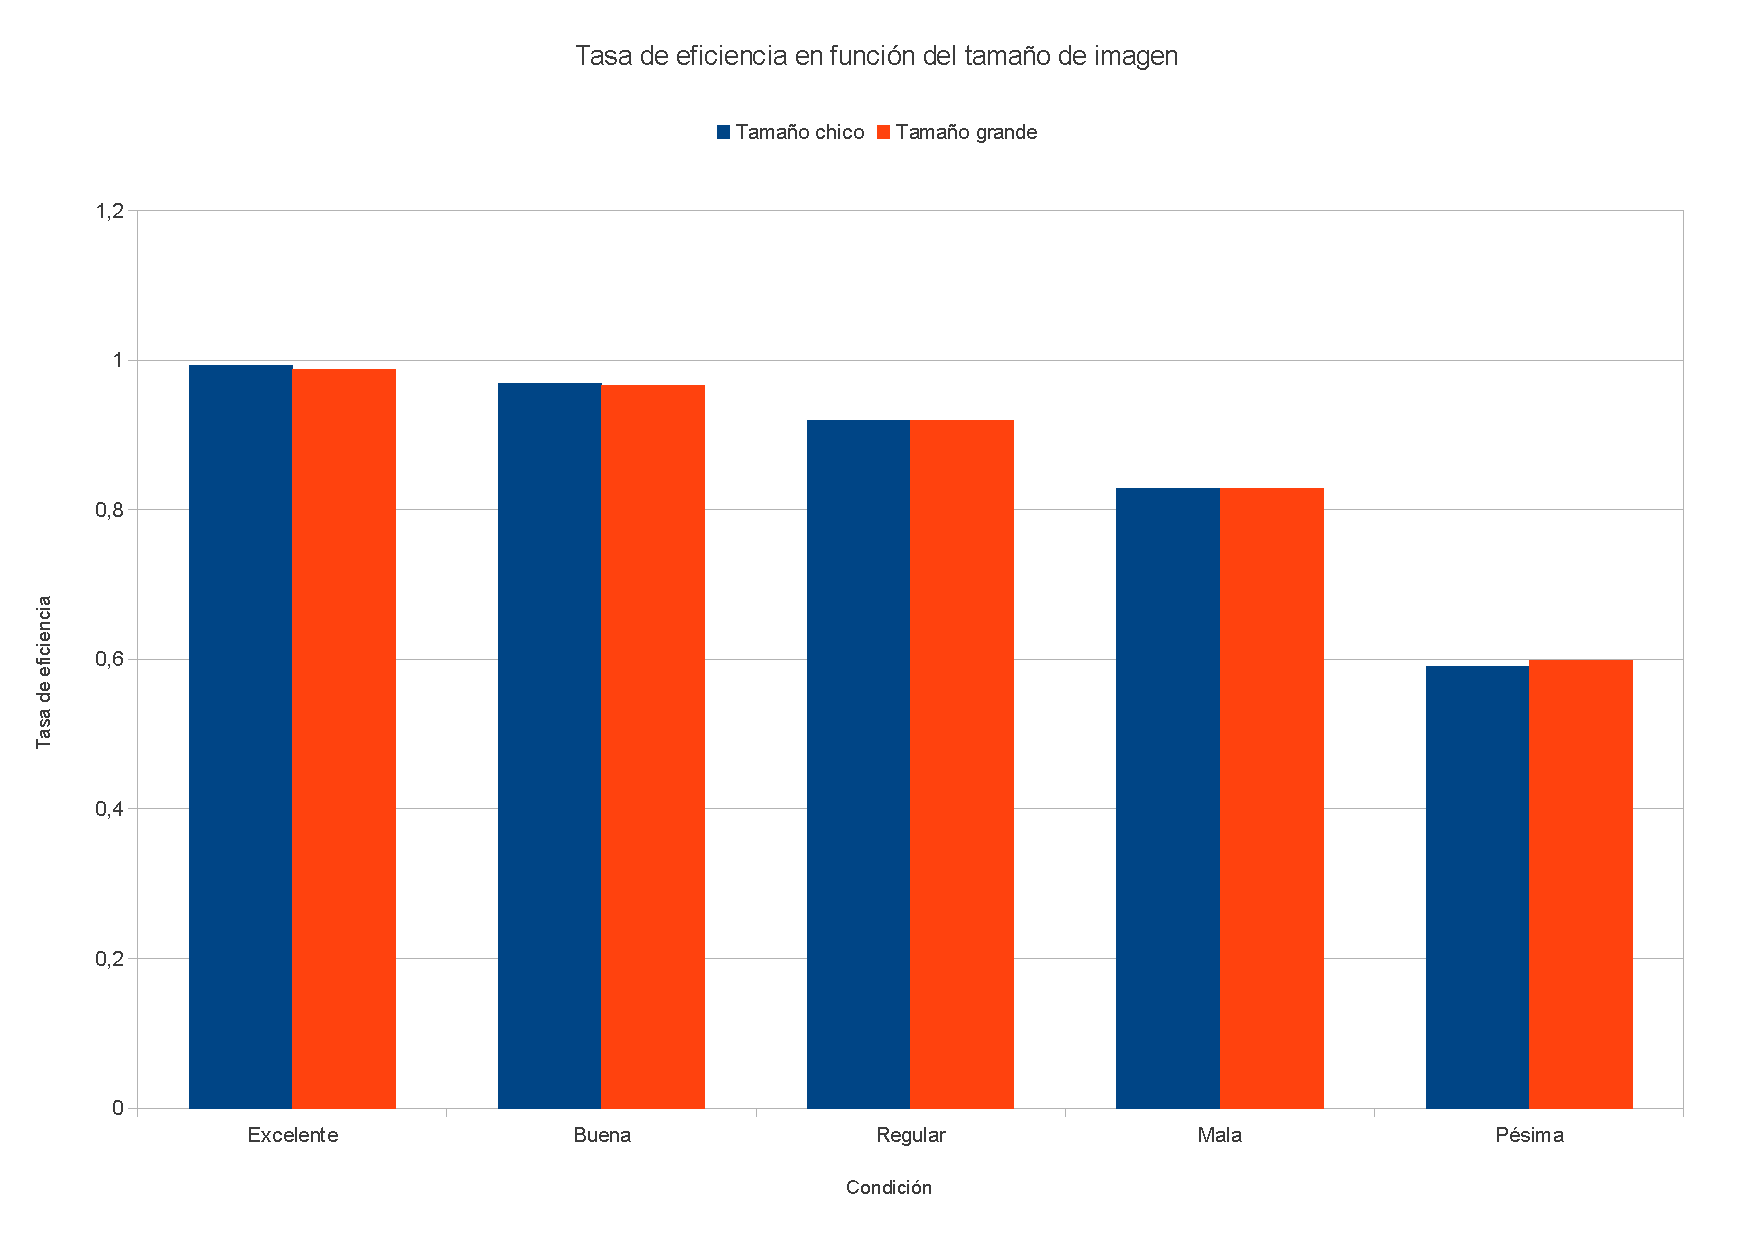
\includegraphics[scale=0.5]{graphs/TEvsRes.pdf}
\caption{Tasa de eficiencia en función de la resolución para distintos escenarios.}
\label{TEvsRes}
\end{figure}
